\documentclass[10pt,conference]{IEEEtran}

\usepackage{xspace,framed}
\usepackage{listings}
\usepackage{graphicx}
\usepackage{epstopdf} %converting to PDF
\usepackage{subfig} 
\usepackage{xcolor,colortbl}
\usepackage{amssymb}
\usepackage{amsmath}
\usepackage{hyperref}
\usepackage{cite}	
\usepackage{mathtools}
\usepackage{tikz}
\usetikzlibrary{positioning, automata, shapes.arrows, calc, shapes, arrows}
\usetikzlibrary{patterns}
\usepackage{pgfplots}

%\setcopyright{acmcopyright}
%\acmDOI{10.475/123_4}
%\acmISBN{123-4567-24-567/08/06}
%\acmConference[ASE '17]{The ACM SIGBED International Conference on Embedded Software }{October 15--20, 2017}{Seoul, South Korea}
%\acmYear{2017}
%\copyrightyear{2017}
%\acmPrice{15.00}

\renewcommand{\baselinestretch}{0.991}
\newcommand\tool{{DSSynth Toolbox}\xspace}
\newcommand{\fwl}[1]{\mathcal{FWL}[#1]}

\begin{document}

\title{DSSynth: An Automated Digital Controller Synthesis Tool for Physical Plants} 
% via MATLAB Toolbox}

\author{\IEEEauthorblockN{Alessandro Abate$^{1}$, Iury Bessa$^{2}$, Dario Cattaruzza$^{1}$, Lennon Chaves$^{2}$, Lucas Cordeiro$^{1,2}$, \\ 
Cristina David$^{1}$, Pascal Kesseli$^{1}$, Daniel Kroening$^{1}$ and Elizabeth Polgreen$^{1}$}
\IEEEauthorblockA{$^{1}$University of Oxford, Oxford, United Kingdom \\
$^{2}$Federal University of Amazonas, Manaus, Brazil}}

%\author{\IEEEauthorblockN{Erickson H. da S. Alves, Lucas C. Cordeiro, Eddie B. de Lima Filho}
%		\IEEEauthorblockA{Federal University of Amazonas, Brazil\\
%			E-mails: erickson.alves@indt.org.br, lucascordeiro@ufam.edu.br, eddie@ctpim.org.br}}
			
\maketitle

\begin{abstract}
We present an automated MATLAB Toolbox, named as DSSynth 
(Digital-System Synthesizer), to synthesize sound digital controllers 
for physical plants that are represented as linear time-invariant
systems with single input and output. In particular, DSSynth synthesizes digital 
controllers that are sound w.r.t. the stability specification by taking into account finite word-length 
effects in their representation. DSSynth considers the complete range
of approximations, including time discretization, quantization effects, 
and finite-precision arithmetic (and its rounding errors). 
Currently, there are two DSSynth versions for synthesizing digital controllers for physical plants 
represented by transfer function or state-space equations: a command-line and 
a MATLAB application. The resulting toolbox 
enables application of program synthesis to real-world control engineering systems.
\end{abstract}

%
% The code below should be generated by the tool at
% http://dl.acm.org/ccs.cfm
% Please copy and paste the code instead of the example below. 
%
\begin{IEEEkeywords}
Formal Synthesis; Digital Control Systems; MATLAB Toolbox; Finite-Word Length; Verification
\end{IEEEkeywords}

%---------------------------------------------------
\section{Introduction}
%---------------------------------------------------

Control theory targets the construction of reliable systems by providing mathematical guarantees about the stability and the desired 
performance of closed-loop dynamics, where outputs of discrete plant $G(z)$ 
are fed back and compared to a reference signal to which a (designed) 
controller $C(z)$ should steer~\cite{astrom1997computer}. 
Fig.~\ref{fig:typical-control-system} shows a typical closed-loop digital control system.
%
\begin{figure}[ht!]
\centering
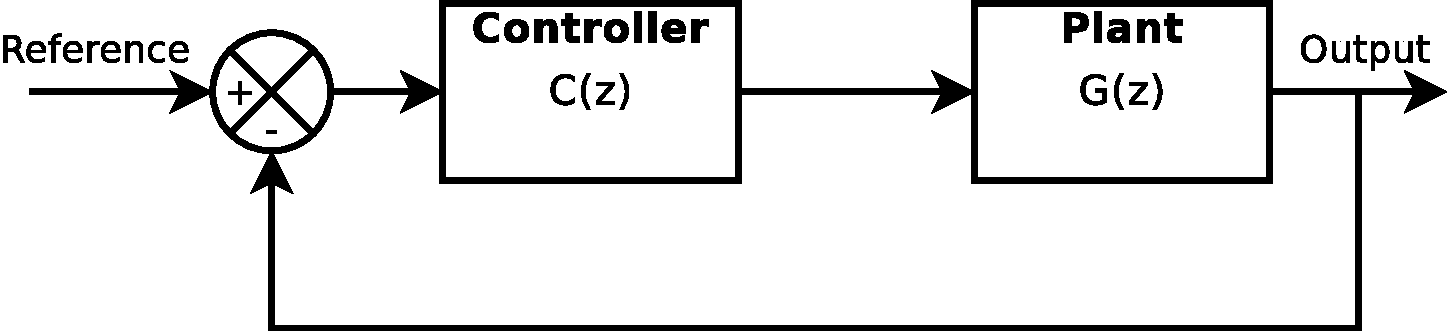
\includegraphics[width=0.4\textwidth]{closedloopseries.pdf}
\caption{Typical Closed-loop Control System.}
\label{fig:typical-control-system}
\end{figure}

%Embedded digital control systems perform computations over digital signals 
%to influence the system behavior~\cite{Ogata2001}; it can be mathematically 
%expressed as difference equations, transfer functions or state-space equations. 
%Here, the focus is on transfer function and state-space representations. 


There are various mathematical representations for control 
systems,  e.g.,  transfer functions and state-space equations (difference or differential equations). 
Here, 
systems with a single input and a single output (SISO) are considered and 
represented by transfer functions or state-space LTI models. LTI models 
are used in several engineering applications to support non-trivial tasks when 
applied to embedded \& cyber-physical systems (e.g., robot manipulator, smart grid, 
power plants, distributed robotics, and automatic pilot avionics). 
The following expression presents the general form 
of a discrete plant or a digital controller based on the transfer function representation:
%
\begin{equation}
\small
\label{eq:transferfunction}
H(z)=\frac{B(z)}{A(z)}=\frac{b_{0}+b_{1}z^{-1}+...+b_{M}z^{-M}}{a_{0}+a_{1}z^{-1}+...+a_{N}z^{-N}},
\end{equation}
%
\noindent where $z^{-1}$ is called the backward-shift operator; $A(z)$ and $B(z)$ are 
the denominator and numerator polynomials; and $N$ and $M$
represent the denominator and numerator polynomials order, respectively.
%
In a state-space form, 
the behavior of a system is represented via a state evolution equation $x(n+1)$ and an instantaneous 
output equation $y(n)$, as follows:
%
\begin{equation}
\begin{split}
x(n+1) &= A x(n) + B u(n)
\\
y(n) &= C x(n) + D u(n), 
\end{split}\label{eq:ss-example}
\end{equation}

\noindent where $A$, $B$, $C$ and $D$ are matrices that fully specify the model. 
%
Controllers synthesis for LTI systems is richly studied 
in the literature~\cite{mazo2010pessoa,DBLP:conf/emsoft/RavanbakhshS16,economakos2016automated}; 
however, there are many challenges when 
digital control system theory is used, mainly due to the finite-word 
length (FWL) effects leading to truncation 
or round-off errors~\cite{Guang2013, Istepanian2001}, time discretization 
and quantization noise, which are typically introduced by Analogue-to-Digital 
(ADC) and Digital-to-Analogue (DAC) conversion~\cite{astrom1997computer}. 

Recently, a new methodology to synthesize digital control systems has been proposed, 
named DSSynth (Digital-System Synthesizer)~\cite{abate2017, abatecav2017}, 
which is based on the Counter-Example Guided Inductive Synthesis 
(CEGIS) approach~\cite{DBLP:conf/asplos/Solar-LezamaTBSS06}. Here, CEGIS is used
as a program synthesis engine that is able to generate sound digital controllers for highly non-trivial 
control system specifications with a very high degree of automation. The program synthesis engine 
uses a specification as starting point, and subsequently produces a sequence of candidate 
programs from a given template. The candidate programs are iteratively refined to eventually 
satisfy the specification. Modern synthesis engines such as the one used here combine automated testing, genetic algorithms 
and SMT-based automated reasoning~\cite{DBLP:journals/corr/AlurFSS16a, DBLP:conf/lpar/DavidKL15}. 
Using the CEGIS-based approach, DSSynth synthesizes stable digital controllers
for a given physical plant represented by either transfer functions or state-space equations~\cite{abate2017,abatecav2017}.

Notably, there are toolboxes in MATLAB with functions and scripts to facilitate the 
digital system design and implementation~\cite{matlab-toolbox}. Indeed, there is a MATLAB 
Toolbox named as DSVerifier Toolbox~\cite{issta2017,DBLP:journals/tc/BessaIPCF17,DBLP:journals/dafes/BessaICF16}, which automatically detects 
specific errors related to digital system design ({\it e.g.}, stability, limit cycle and overflow) 
using symbolic model checking techniques based on Boolean Satisfiability (SAT) and 
Satisfiability Modulo Theories (SMT) solvers. Pessoa~\cite{mazo2010pessoa} is another 
toolbox, but applied to the synthesis of correct-by-design digital controllers. 
In particular, Pessoa is based on approximate bisimulation, which allows control engineers to replace differential equations, 
describing a physical plant, by a respective finite-state machine. However, Pessoa does not take advantage of
recent advances in bit-accurate verification of programs to synthesize controllers w.r.t. FWL effects. MATLAB already offers a tool 
named as Control System Tuner~\cite{autotuner} for automatically designing controllers based on optimization solvers or graphical analysis. 
However, the Control System Tuner is unable to consider FWL effects during the controller synthesis process.
To the best of our knowledge, there is no MATLAB toolbox able to perform digital controller synthesis based on 
program synthesis engines that considers the complete range of approximations, including time discretization, 
quantization effects, and finite-precision arithmetic and its rounding errors. 

The present tool paper addresses this limitation and describes a toolbox for the DSSynth tool~\cite{abate2017, abatecav2017} 
in a MATLAB environment, named \tool. The main advantage for the use of a MATLAB toolbox 
lies on designing physical plants in MATLAB and then promptly synthesizing a stable and safe digital controller,
considering the complete range of approximations. 
Notably, when using the \tool, an engineer is able to model a physical plant with MATLAB
through transfer function or state-space representations, considering low-level systems parameters 
(implementation features and numerical format).

%---------------------------------------------------
\section{Counterexample-Guided Inductive Synthesis for Control Systems}
\label{sec:CEGIS}
%---------------------------------------------------

%\textcolor{red}{Cristina: can you please generalize our CEGIS implementation for control here?}

%% The input specification provided to the program synthesizer is of the form
%% $\exists P .\, \forall a.\, \sigma(a, P)$, where $P$ ranges over functions
%% (where a function is represented by the program computing it),
%% $a$ ranges over ground terms, and $\sigma$ is a quantifier-free formula. 
%% We~interpret the ground terms over some finite domain~$\mathcal{D}$.

The design of our synthesizer consists of two main phases, an inductive
synthesis phase, {\sc synthesise}, and a validation phase, {\sc verify},
which interact via a finite set of test vectors that is updated
incrementally.  Given a stability and safety specification, the
inductive synthesis procedure tries to find a candidate solution
satisfying the specification for the given set of test inputs.
%
If the synthesis phase succeeds in finding a witness, this witness is
a candidate solution to the full synthesis formula.  We pass this
candidate solution to the validation phase, which checks whether it is
a full solution (i.e., satisfies the specification for all possible
inputs).  If this is the case, then the algorithm terminates.
Otherwise, additional information is provided to the inductive
synthesis phase in the form of a new counterexample, C-ex, that is added to
the set of test inputs, and the loop iterates again.

We use two different instantiations of the synthesiser
in order to find stable and safe digital
controllers. The two approaches differ in
the manner in which they check the safety specification
for all reachable states.

%%%%%%%%%%%%%%%%%%%%%%%%%%%%%%%%%%%%%%%%%%%%%%%%%%%%%%%%%%%%%%%%%%%%%%%%%%
\begin{figure}[htb]
{\scriptsize
\centering
\resizebox{.43\textwidth}{!}
{
  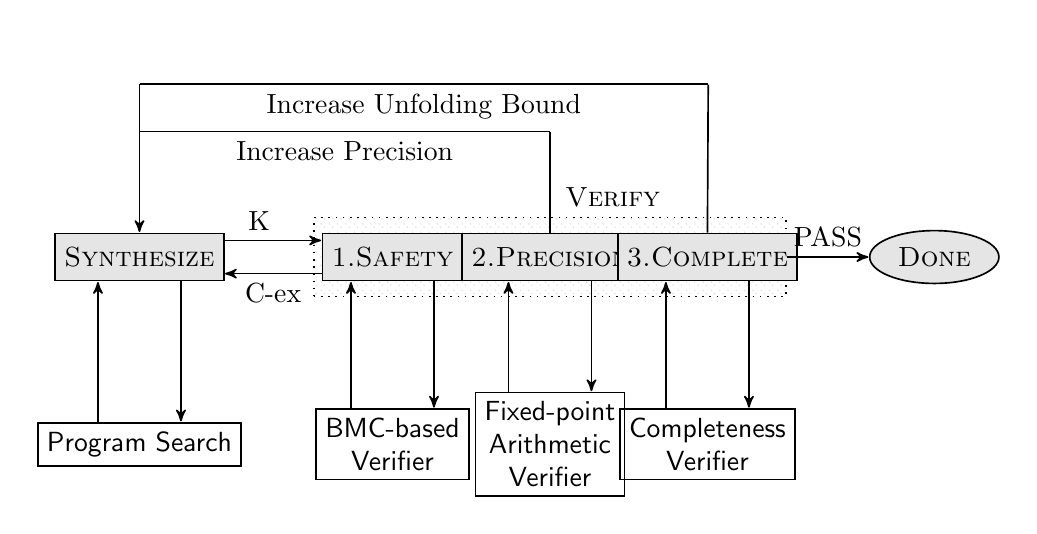
\begin{tikzpicture}[scale=0.3,->,>=stealth',shorten >=.2pt,auto, semithick, initial text=, ampersand replacement=\&,]
  \matrix[nodes={draw, fill=none, shape=rectangle, minimum height=.2cm, minimum width=.2cm, align=center
},
          row sep=.6cm, column sep=.9cm] {
   \coordinate (aux1);
   \& \coordinate (aux2);
   \&;\\
   \coordinate (aux3);
   \& \coordinate (aux4);
   \&;\\
   \coordinate (aux5);
   \& \coordinate (aux6);
   \&;\\
   \node[minimum width=1.5cm, minimum height=0.6cm, fill=gray!20] (synth) {{\sc Synthesize}};
   \&
   complexnode/.pic={ 
     \node[rectangle,draw,dotted,
	minimum width=6cm,
	minimum height=1cm,
        pattern=north west lines, pattern color=gray!20,
	label={\sc ~~~~~~~~~~~~Verify},] (verif) {};
     \node[minimum width=1cm, minimum height=0.6cm, fill=gray!20] (verif1) at ([xshift=-2cm]verif.center) {{\sc 1.Safety}};
     \node[minimum width=1cm, minimum height=0.6cm, fill=gray!20] (verif2) at ([xshift=0cm]verif.center) {{\sc 2.Precision}};
     \node[minimum width=1cm, minimum height=0.6cm, fill=gray!20] (verif3) at ([xshift=2cm]verif.center) {{\sc 3.Complete}};
     %\node[minimum width=1cm, minimum height=0.6cm, fill=gray!20] (verif4) at ([xshift=3.1cm]verif.center) {{\sc 5.Sampling}};
   } 
   \& \node[ellipse, fill=gray!20] (done) {{\sc Done}};\\
   \& \\
   \node[minimum height=0cm] (gp) {\sf Program Search};
   \&
   complexnode/.pic={ 
     \coordinate (aux);
   \node (bmc) at ([xshift=-2cm]aux.center) {\sf BMC-based \\ \sf Verifier};
   \node (fp)  at ([xshift=0cm]aux.center) {\sf Fixed-point \\ \sf Arithmetic\\ \sf Verifier};
   \node (sv)  at ([xshift=2cm]aux.center) {\sf Completeness\\ \sf Verifier};
   %\node (cv)  at ([xshift=3.1cm]aux.center) {\sf Sampling\\Verifier};
   }   
    \\
  };

   \path
    ([yshift=2em]synth.east) edge node[xshift=-0.5em,align=center] {K} ([yshift=2em]verif1.west)
    ([yshift=-2em]verif1.west) edge node {C-ex} ([yshift=-2em]synth.east)
    ([xshift=-5em]fp.north) edge node[align=center]  {} ([xshift=-5em]verif2.south)
    ([xshift=-5em]sv.north) edge node[align=center]  {} ([xshift=-5em]verif3.south)
    %([xshift=-5em]cv.north) edge node[align=center]  {T/F} ([xshift=-5em]verif4.south)
    ([xshift=5em]verif1.south) edge node[align=center] {} ([xshift=5em]bmc.north)
    ([xshift=5em]verif2.south) edge node[align=center] {} ([xshift=5em]fp.north)
    ([xshift=5em]verif3.south) edge node[align=center] {} ([xshift=5em]sv.north)
    %([xshift=5em]verif4.south) edge node[align=center] {$K$} ([xshift=5em]cv.north)
    ([xshift=-5em]bmc.north) edge node[align=center]  {} ([xshift=-5em]verif1.south)
    (verif) edge node {PASS} (done)
    ([xshift=5em]synth.south) edge node[align=center] {} ([xshift=5em]gp.north)
    ([xshift=-5em]gp.north) edge node[align=center] {} ([xshift=-5em]synth.south)
    (aux3) edge (synth.north);
   \path[-]
   (verif2.north) edge node[align=center] {} ([xshift=0cm]aux6)
   ([xshift=0cm]aux6) edge node[align=center] {Increase Precision} (aux5)
   (verif3.north) edge node[align=center] {} ([xshift=6.7cm]aux4)
   ([xshift=6.7cm]aux4) edge node[align=center] {Increase Unfolding Bound} (aux3);
   %(verif4.north) edge node[align=center] {} ([xshift=10.5cm]aux2)
   %([xshift=10.5cm]aux2) edge node[align=center] {Increase Sampling Rate} (aux1);

 \end{tikzpicture}
}}
\caption{CEGIS with multi-staged verification}
\label{fig:CEGIS-precision-increment}
\end{figure}

%%%%%%%%%%%%%%%%%%%%%%%%%%%%%%%%%%%%%%%%%%%%%%%%%%%%%%%%%%%%%%%%%%%%%%%%%%%

The first approach, presented in Fig.~\ref{fig:CEGIS-precision-increment}, 
uses a multi-staged verification process. 
It starts by devising a digital controller that stabilizes the model while remaining safe for a
pre-selected time horizon ($k$) and a single initial state; then, it
employs a multi-staged verification process as follows:
(i) The first verification stage ({\sc safety}) checks that the candidate
solution, which we synthesized to be safe for at least one initial
state, is safe for \emph{all} possible initial states, i.e., does not reach
an unsafe state within $k$ steps.
(ii) The second verification stage ({\sc precision})
 restores soundness with respect to the plant precision
by using interval arithmetic \cite{moore1966interval} to validate the 
operations performed by the previous stage. 
(iii) The third verification stage ({\sc complete}) checks that the current
$k$ is large enough to ensure safety for any $k'{>}k$.  Here, we compute the
completeness threshold $\overline{k}$ for the current candidate controller 
$K$~\cite{abatecav2017}, i.e., the number of
iterations required to sufficiently unwind the closed-loop state-space
model such that the boundaries are not violated for any larger number of
iterations, and
check that $k{\geq}\overline{k}$.

\begin{figure}
\centering
{\scriptsize
  \resizebox{.5\textwidth}{!}
  {
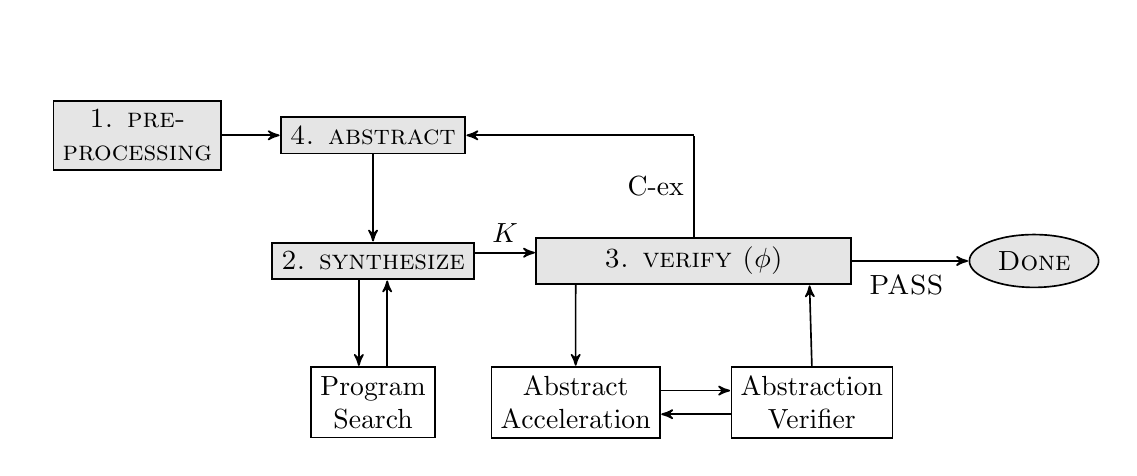
\begin{tikzpicture}[scale=0.3,->,>=stealth',shorten >=.2pt,auto, semithick, ampersand replacement=\&,]
  \matrix[nodes={draw, fill=none, shape=rectangle, minimum height=.2cm, minimum width=.2cm, align=center},row sep=.8cm, column sep=.2cm] {
   \coordinate (aux1);
   \& \coordinate (aux2);
   \& ;\\
   \&\node[fill=gray!20,align=center,xshift=-1.5cm] (pre) {{\sc 1. pre-}\\{\sc processing}};
   \& \node[fill=gray!20,align=center] (abstract) {\sc 4. abstract};
   \& \coordinate (aux); \\ 
   \&
   \& \node[fill=gray!20,align=center] (synth) {\sc 2. synthesize};
   \& \node[fill=gray!20,align=center, minimum width=4cm] (verify) {\sc 3. verify ($\phi$)};
      \node[draw=none] (SAT) at ([xshift=2.7cm,yshift=-.3cm]verify)  {\sc PASS};
   \& \node[ellipse, fill=gray!20] (done) {{\sc Done}};\\
   \&
   \& \node[draw,rectangle,align=center] (KSAT) {Program \\ Search};
   \& complexnode/.pic={
     \coordinate (AA);
     \node[draw,rectangle,align=center] (AAV) at ([xshift=-1.5cm]AA.center) {Abstract\\Acceleration};
     \node[draw,rectangle,align=center] (AAC) at ([xshift=1.5cm]AA.center) {Abstraction \\ Verifier};
    }\\
  };
  \path
    (pre.east) edge node[align=center] {} (abstract.west)
    (abstract.south) edge node{} (synth.north)
    ([yshift=1em]synth.east) edge node {$K$} ([yshift=1em]verify.west)
    (aux) edge (abstract.east) 
    (verify.east) edge (done.west);
  \path
    ([xshift=+.6cm]KSAT.north) edge[left] node[xshift=-.3cm] {} ([xshift=0.6cm]synth.south) 
    ([xshift=-.6cm]synth.south) edge node[align=center,xshift=.3cm] {} ([xshift=-.6cm]KSAT.north)
    ([yshift=.5cm]AAV.east) edge node{} ([yshift=.5cm]AAC.west)
    ([yshift=-.5cm]AAC.west) edge node{} ([yshift=-.5cm]AAV.east)
    (AAC.north) edge node{} ([xshift=4.9cm]verify.south)
    ([xshift=-5cm]verify.south) edge node{} (AAV.north);
  \path[-] 
     (verify.north) edge node {C-ex} (aux);
\end{tikzpicture}
}
}
\caption{Abstraction-based CEGIS}
\label{fig:CEGARIS} 
\end{figure}

Instead of unfolding the dynamics, the second approach (shown in Fig.~\ref{fig:CEGARIS}) 
employs {\em abstract acceleration}~\cite{cattaruzza2015unbounded} to 
simultaneously evaluate all possible progressions of the model. This eliminates the need for
a completeness threshold, since the time horizon considered in abstract acceleration is infinite.
An additional preprocessing phase is used to compute 
a set of initial bounds on $K$ based on input constraints. 
Note that these bounds will be used by the {\sc synthesize} phase to reduce the size of the solution space.
%
Since this model is based on abstraction, we initially perform the synthesis over a basic
model that abstracts away the complexity of the specification and is only refined to a more
complex model when a counterexample is found. 
% Thus, we may only look at the gain of the
% model to synthesise a controller and to add further restrictions on specific sections of the reach
% tube when these prove to invalidate the solution.
The use of this Counterexample-Guided 
Abstraction-Refinement results in much faster synthesis and verification since it is applied to
both phases, allowing for faster results whilst maintaining soundness for an infinite time horizon.
 
%\textcolor{red}{We have to talk about the naive and AA back-ends, which are based on our CEGIS framework}

%---------------------------------------------------
\section{Synthesizing Digital Controllers with \tool}
%---------------------------------------------------

%---------------------------------------------------
\subsection{\tool Architecture}
%---------------------------------------------------

The proposed synthesis methodology for closed-loop digital control
systems is based on the DSSynth tool~\cite{abate2017, abatecav2017}, 
which can be split into two main stages as follows: manual (user) and 
automated (DSSynth) procedures, as illustrated in Fig.~\ref{fig:synthesis-flow}. 
%
\begin{figure}[ht!]
\centering
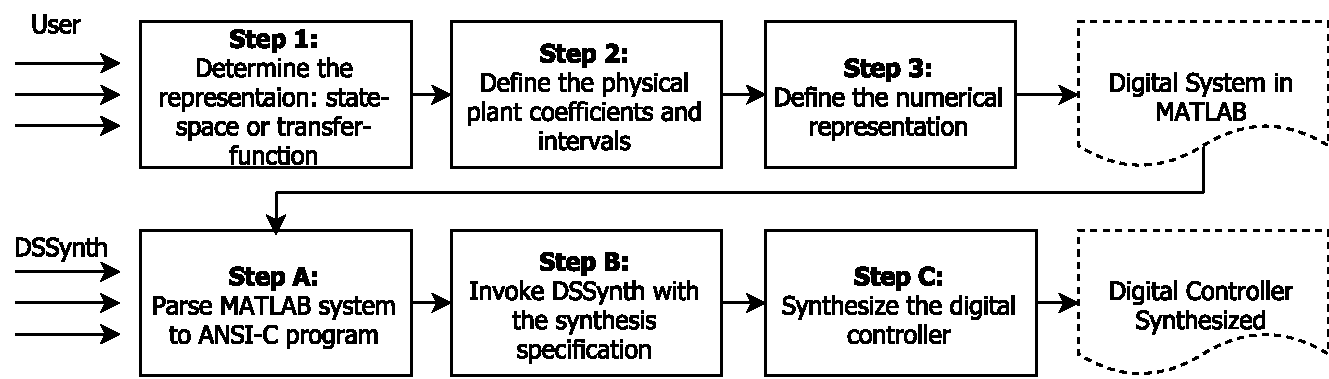
\includegraphics[width=0.45\textwidth]{synthesis-flow.pdf}
\caption{Digital Controller Synthesis Methodology.}
\label{fig:synthesis-flow}
\end{figure}

In step $1$, the user has to define the digital controller representation, 
which can be a transfer function or a state-space model. 
In step $2$, the physical plant (represented by Equations (\ref{eq:transferfunction}) 
or (\ref{eq:ss-example})) must be designed, using a method selected 
from the control literature~\cite{astrom1997computer}. Finally, in step $3$, 
the numerical representation for the digital controller implementation must be 
defined by the user, {\it i.e.}, the FWL format that includes the number of bits for the integer 
and fractional parts as well as the dynamic range inputs. The result of the manual 
procedure performed by the user is a digital system specification for the given 
physical plant in MATLAB. 

After that, the synthesis process starts in step $A$, when \tool obtains the digital system 
specification in MATLAB, and then translates it into an ANSI-C program. 
In step $B$, our CEGIS engine is invoked to synthesize the digital controller w.r.t. the digital system
specification. Finally, in step $C$, the synthesized digital controller considering FWL effects is produced. 
The output generated by \tool is the synthesized digital controller represented either in transfer function 
or state-space equation. The synthesis is considered to be \emph{successful} if a digital controller is correctly 
synthesized w.r.t. FWL effects; otherwise, if any parameter is incorrectly defined in previous steps, 
or if there is no solution (digital controller) for the respective physical plant (given the digital controller
 implementation aspects), then the synthesis is considered to have \emph{failed}.

Our CEGIS engine is implemented as an integrated module within the C bounded model checker (CBMC)~\cite{cbmc}.  CBMC
transforms the ANSI-C representation of our closed-loop control system model into its internal format called
\emph{GOTO}.  We instrument this internal \emph{GOTO} program for each synthesis or verification scenario accordingly,
and use CBMC as an oracle to answer our queries.  CBMC itself relies on an underlying SAT or SMT solver to solve the
resulting formulae.  We model FWL effects, time discretization and the presence of quantization noise explicitly using CBMC's  
nondeterminism API (e.g., \texttt{nondet}, \texttt{CPROVER\_assume} intrinsic functions).  Our module was included in CBMC~5.7 and is available for
public download.\footnote{\url{https://github.com/diffblue/cbmc/archive/cbmc-5.7.zip}}  We further created a VirtualBox OVA image
with our tool pre-installed, including our MATLAB-generated benchmarks and benchmark shell script with instructions
to run all benchmarks and reproduce our
experiments.\footnote{\url{www.cprover.org/DSSynth/controller-synthesis-cav-2017.tar.gz}}  The current development branch
of our toolbox is available in a public GitHub
repository.\footnote{\url{https://github.com/ssvlab/dsverifier/tree/master/toolbox-dssynth}}

The entire implementation consists of $400$ lines of MATLAB scripts for the UI
module, $585$ and $800$ lines of C code in the naive and abstract accelerator
back-ends, respectively (cf.~Section~\ref{sec:CEGIS}).  $4000$ lines of C code for utility functions such as
interval and fixed-point arithmetic, as well as $1000$ lines of C++ code in the
control synthesis module in CEGIS CBMC.  We evaluate \tool using $18$ SISO 
control system benchmarks. Additionally, the documentation and videos about \tool are available 
at \url{http://dsverifier.org/dsverifier/dssynth-toolbox/}.


%---------------------------------------------------
\subsection{\tool Procedures}
%---------------------------------------------------

The \tool performs the following automated procedures 
to synthesize a given digital controller:

\begin{enumerate}
\item \textbf{Setup}: obtains the physical plant, fixed-point format 
and dynamic input ranges, and translates them to a specific structure in MATLAB.
\item \textbf{Parse}: obtains the digital system specification and translates 
it into an ANSI-C program.
\item \textbf{Execution}: obtains the ANSI-C program from the previous (parse) step 
and calls our CEGIS engine as a back-end program synthesis tool to perform the automated synthesis;
\item \textbf{Extraction}: obtains the ``.log'' file that is generated 
after the synthesis phase and then checks the synthesized digital-controller.
\item \textbf{Report}: obtains the digital controller from the previous (extraction) step 
and translates it into the MATLAB structures to show the respective result to the user.
\end{enumerate}

%---------------------------------------------------
\subsection{\tool Features}
%-----------------------------------------------

The \tool's features can be described as follows:

\begin{itemize}
\item \textbf{Representation}: the synthesis can be 
performed for digital systems specified via 
transfer function or as state-space models.
\item \textbf{Fixed-Point Arithmetic}: the digital 
controller is synthesized considering FWL effects, 
using the given fixed-point numerical representation.
\item \textbf{Interface}: the synthesis can be executed 
via command-line or graphical-user interface (GUI). 
For the GUI application, the user can plot the step response 
to reproduce the stability in closed-loop of the synthesized digital controller.
\end{itemize}

%---------------------------------------------------
\subsection{\tool Usage}
%---------------------------------------------------

%---------------------------------------------------
\subsubsection{Command Line Version}
%---------------------------------------------------

Users must provide a digital system described as a MATLAB model 
using a \texttt{tf} (for transfer function) or an \texttt{ss} (for state-space model) 
command (cf. step $1$ of Fig.~\ref{fig:synthesis-flow}).
\tool is called via command line in MATLAB as 

\begin{center} 
\texttt{synthesize(plant, intBits, fracBits, maxR, minR)}
\end{center} 

\noindent where \texttt{plant} is the physical plant in state-space or transfer function representation, 
\texttt{intBits} is the integer part, \texttt{fracBits} is the fractional part, \texttt{maxR} and \texttt{minR} 
are the maximum and minimum dynamic range, respectively (cf. steps $2$ and $3$ of Fig.~\ref{fig:synthesis-flow}).
%
After executing the \texttt{synthesize} command in MATLAB, 
\tool provides the synthesized digital controller, according to the digital system representation. 

%---------------------------------------------------
\subsubsection{MATLAB Application Version} 
%---------------------------------------------------

A graphical user interface application was developed (as shown in Fig.~\ref{fig:gui-for-tf}) 
to favor digital controller synthesis in MATLAB. Its aim is to improve usability and, 
consequently, to attract more digital dynamical system engineers. Users can provide all 
required parameters for digital controller synthesis: physical plant specification, 
fixed-point representation and dynamic inputs. 
%
\begin{figure}[ht]
    \centering
    \subfloat[Define the system representation and the physical plant.]{
		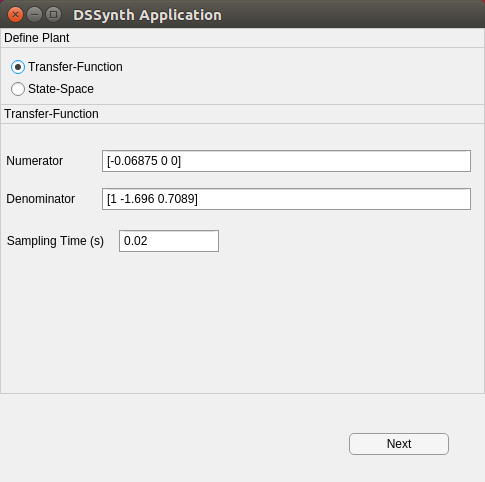
\includegraphics[width=0.2\textwidth]{step1.png}
		\label{step1}}
		\hfil
    \subfloat[Define implementation aspects and dynamic range.]{
	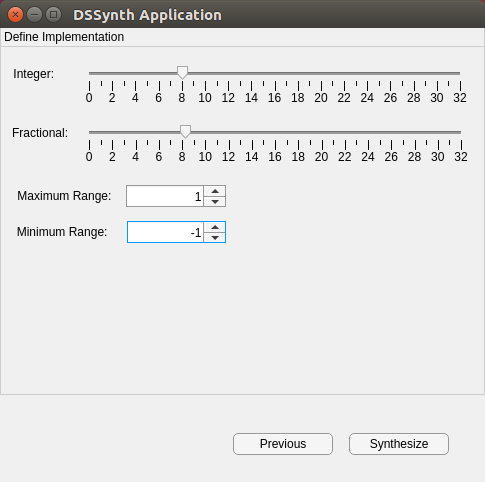
\includegraphics[width=0.2\textwidth]{step2.png}
		\label{step2}}
		\hfil
    \subfloat[Resulting digital controller synthesized by DSSynth.]{
	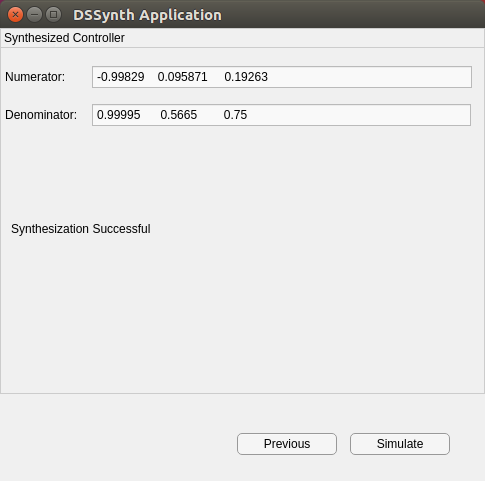
\includegraphics[width=0.2\textwidth]{step3.png}
		\label{step2}}
		\hfil
    \subfloat[Step response for the synthesized digital controller.]{
	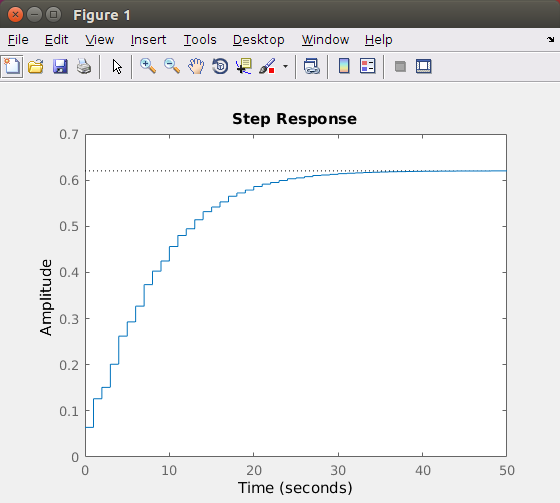
\includegraphics[width=0.22\textwidth]{step4.png}
		\label{step3}}
		\hfil
    \caption{DSSynth GUI application for the controller synthesis based on transfer function representation.}
    \label{fig:gui-for-tf}
\end{figure}

%---------------------------------------------------
\subsection{Illustrative Example}
%---------------------------------------------------

To illustrate the \tool's usage, Fig.~\ref{toolbox-usage} shows each step of the 
synthesis process for a physical plant described in Eq.~\eqref{equation_plant},
which represents a real unmanned aerial vehicle (UAV) quadcopter system~\cite{bouabdallah}. 
This physical plant is expressed by a transfer function $G(z)$, where 
$B(z)$ and $A(z)$ represent the numerator and denominator, respectively, as
%
\begin{equation}
\label{equation_plant}
G(z)=\frac{B(z)}{A(z)}=\frac{-0.06875z^{2}}{z^2-1.696z+0.7089}.
\end{equation}

\begin{figure}[ht]
\scriptsize
\begin{lstlisting}[xleftmargin=.025\textwidth,xrightmargin=.025\textwidth, frame=single,]
>> num = [-0.06875 0 0];
>> den = [1.0000 -1.696 0.7089];
>> system = tf(num,den,0.002);
>> y = synthesize(system,8,8,1,-1);
>> SYNTHESIS SUCCESSFUL
>> y = 
>>  -0.9983z^2 + 0.09587z + 0.1926
>>  --------------------------------
>>       z^2 + 0.5665z + 0.75
\end{lstlisting}
\vspace{-0.2cm}
\caption{Synthesis of a digital controller for the physical plant defined in Eq.(\ref{equation_plant}) in MATLAB, with a fixed-point format  $\left\langle 8,8\right\rangle$.}
\label{toolbox-usage}
\end{figure}

In Fig.~\ref{toolbox-usage}, ``num'' represents $B(z)$ and ``den'' represent $A(z)$, while 
$y$ represents the synthesized stable digital controller, which is defined by Eq.(\ref{equation_controller}).
%
\begin{equation}
\label{equation_controller}
C(z)=\frac{-0.9983^{2}+0.09587z+0.1926}{z^2+0.5665z+0.75}.
\end{equation}

A digital system is stable \textit{iff} all of its poles are inside the $z$-plane unity circle, 
namely poles must have the modulus less than one~\cite{astrom1997computer}. In order to compute the poles for the digital 
system represented by Equations~\eqref{equation_plant} and \eqref{equation_controller}, 
the user can invoke the \texttt{feedback} and \texttt{series} commands in MATLAB~\cite{matlab-toolbox} 
to achieve a general equation regarding the transfer function representation, as illustrated in Fig.~\ref{combine-controller-plant}. 

\begin{figure}[ht]
\scriptsize
\begin{lstlisting}[xleftmargin=.025\textwidth,xrightmargin=.025\textwidth, frame=single,]
>> num = [-0.99832 0.09587 0.1926];
>> den = [1 0.5665 0.75];
>> controller = tf(num,den,0.002);
>> num = [-0.06875 0 0];
>> den = [1.0000 -1.696 0.7089];
>> plant = tf(num,den,0.002);
>> sys = feedback(series(controller, plant),1)
>> sys =
>>        0.06863z^4 - 0.006591z^3 - 0.01324z^2
>> ---------------------------------------------------
>> 1.069z^4 - 1.136z^3 + 0.4849z^2 - 0.8704z + 0.5317
\end{lstlisting}
\vspace{-0.2cm}
\caption{General equation for the closed-loop control system using the series configuration as shown in Fig.~\ref{fig:typical-control-system}.}
\label{combine-controller-plant}
\end{figure}

The general equation that represents the closed-loop control system, using the series configuration as shown in Fig.~\ref{fig:typical-control-system},
is described by Equation~\ref{equation_general} as follows
%
\begin{equation}
\small
\label{equation_general}
\frac{N(z)}{D(z)}=\frac{0.06863z^{4} - 0.006591z^{3} - 0.01324z^{2}}{1.069z^{4} - 1.136z^{3} + 0.4849z^{2} -0.8704z + 0.5317}.
\end{equation}
 
For the stability check, if any root of the denominator polynomial $D(z)$ in Equation~\ref{equation_general} 
has modulus equal or greater than one, then the system is unstable; 
otherwise, it is stable. Indeed, the roots computed by the function \texttt{roots} 
in MATLAB~\cite{matlab-toolbox} result in the following poles as shown in Fig.~\ref{roots-of-dz}, 
which means that DSSynth has synthesized a stable digital controller.

\begin{figure}[ht]
\scriptsize
\begin{lstlisting}[xleftmargin=.025\textwidth,xrightmargin=.025\textwidth, frame=single,]
>> den = [1.069 -1.136 0.4849 -0.8704 0.5317]
>> r = roots(den)
>> r =
>>  -0.2912 + 0.8061i
>>  -0.2912 - 0.8061i
>>   0.8225 + 0.0219i
>>   0.8225 - 0.0219i
\end{lstlisting}
\vspace{-0.2cm}
\caption{Roots of the polynomial $D(z)$ given by Equation~\ref{equation_general}.}
\label{roots-of-dz}
\end{figure}

Simulating the digital system represented by Equations \eqref{equation_plant} and \eqref{equation_controller} 
to validate and reproduce the system stability, the user can invoke the step response using the 
command \texttt{dstep} in MATLAB, and then observe that the plotted graph shows a stable digital system, 
as shown in Fig.~\ref{step-response}.
%
\begin{figure}[ht]
  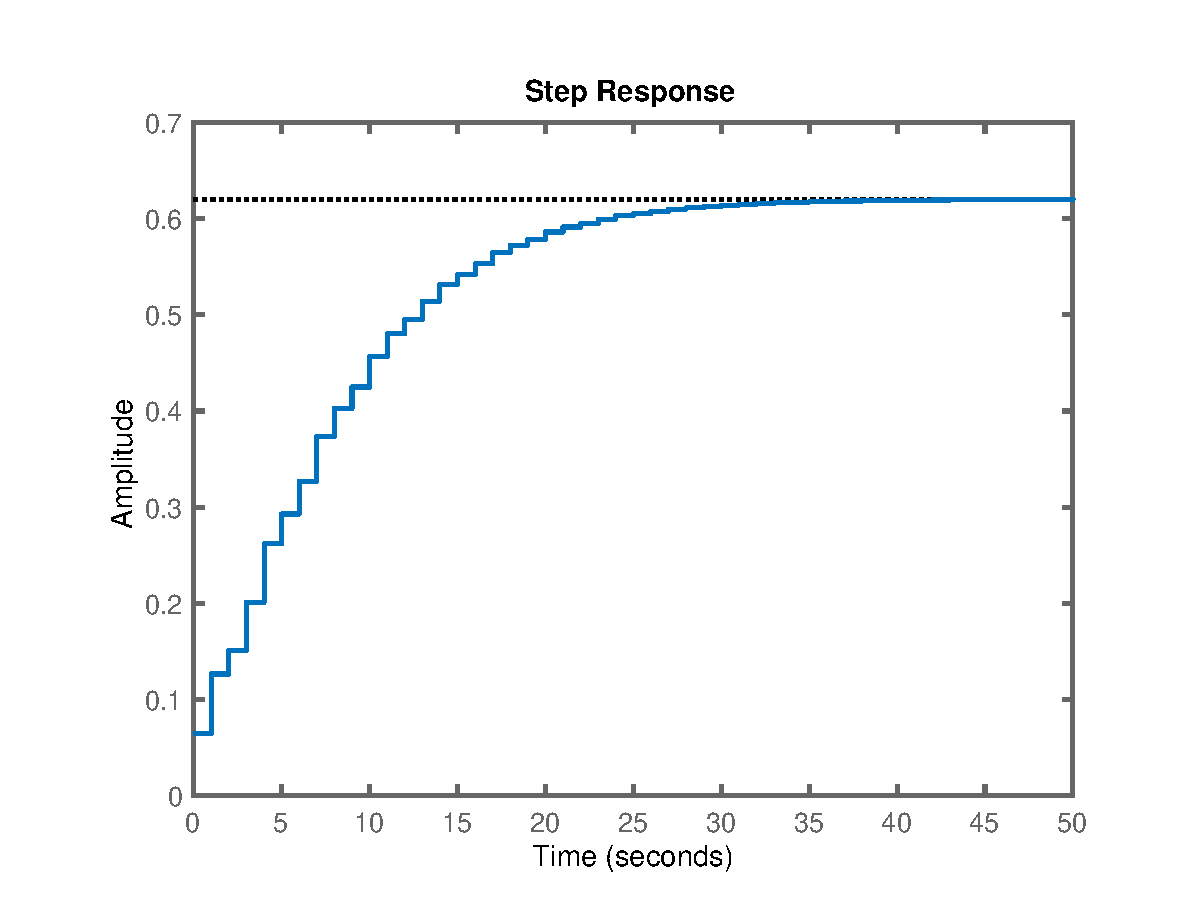
\includegraphics[width=0.5\textwidth]{step-response.eps}
  \caption{Step response for the Eq.~\eqref{equation_plant} describing a stable system for the UAV quadcopter system.}
  \label{step-response}
\end{figure}

%---------------------------------------------------
\section{\tool Experimental Evaluation}
%---------------------------------------------------

%---------------------------------------------------
\subsection{Benchmarks Description}
\label{benchmarks-description}
%---------------------------------------------------

Our experimental evaluation consists of $18$ SISO control system benchmarks 
extracted from the literature~\cite{abate2017,abatecav2017,bouabdallah, acrobot,cstr,KOKOTOVIC198023,gajic2008optimal,Franklin15, maglev, converters, CTMS,DBLP:journals/tc/BessaIPCF17,DBLP:journals/dafes/BessaICF16},
which include physical plants for unmanned aerial vehicle (UAV), cruise control system, 
spring-mass damper, satellite, direct current (DC) servo motor, helicopter, 
inverted pendulum, pendulum, magnetic suspension, magnitezed pointer, 1/4 car suspension, 
computer tape driver, flexible beam, guidance system, USCG cutter tampa, continuous stirred tank reactor, 
voltage regulator, and an acrobot control system.

%The first set of benchmarks uses the discrete model of a cruise control system for a car, and accounts for rolling friction, aerodynamic drag, and the gravitational disturbance force. %cruise-control
%The second set of benchmarks considers the discrete model of a simple spring-mass damper plant. %spring-mass damper
%A third set of benchmarks uses the discrete model for satellite attitude dynamics, which require attitude control for orientation of antennas and sensors w.r.t. Earth. %satellite
%The fourth and fifth set of benchmarks describe the discrete model of a DC servo motor velocity dynamics. %servor-motor
%The fifth set of benchcmarks corresponds an USCG cutter Tampa Heading Angle that describes the heading angle  dynamics of a Coast Guard cutter.
%The sixth set of benchmarks contain a flexible beam system that is a plant usually employed in vibration studies. It is  composed by a flexible metallic structure with piezoceramic actuators and sensors.%flexible beam
%The seventh set of benchmarks describes the discrete model for the Helicopter Longitudinal Motion, which provides the longitudinal motion dynamics of a helicopter. %helicopter
%The eighth set of benchmarks contains the discrete model for the known Inverted Pendulum, which describes a pendulum dynamics with its center of mass above its pivot point. %inverted pendulum
%The ninth set of benchmarks contains the Magnetic Suspension discrete model, which describes the dynamics of a mass that levitates with support only of a magnetic field. %magnetic suspension
%The tenth set of benchmarks contains the Computer Tape Driver discrete model, which describes a system to read and write data on a storage device. %tape driver
%The eleventh set of benchmarks contains the unmanned aerial vehicle (UAV) discret model, in particular, a quadrotor attitude system. %uav
%The twelfth set of benchmarks contains the 1/4 Car Suspension plant presents a physical model that connects a car to its wheels and allows relative motion between both parts. %1/4 car suspension
%The thirteenth set of benchmarks contains the Magnetized Pointer plant describes a physical model employed in analogue gauges and indicators that is rotated through interaction with magnetic fields. %magnitezed pointer
%The fourteenth set of benchmarks contains the pendulum which is system composed by a swinging point mass suspended from  a frictionless pivot through a negligible mass rod. %pendulum
%The fifteenth set of benchmarks  contains the Acrobot benchmark corresponds to the model of an two-link  underactuated robot manipulator, named Acrobot, linearized by partial  feedback linearization~\cite{acrobot}. %acrobot
%The sixteenth set of benchmarks contains a voltage regulator benchmark~\cite{KOKOTOVIC198023} that consists in a linear model of a synchronous machine connected to an  infinite bus.
%The seventeenth set of benchmarks contais a continuous stirred tank reactor which describes a linear model for PH dynamics of a PH  neutralization process of an aqueous solution of sodium acetate with  hydrochloric acid in a continuous flow stirred-tank reactor.%cstr
%And finally, the last set of benchmarks contaians the Guidance Control System benchmark which is another high-order system  model used by Chen et al.~\cite{CHEN1979389}  in order reduction  techniques. Guidance systems are used to determine the path of an autonomous vehicle movement.

%-----------------------------------
\subsection{Experimental Setup}
\label{experimental-setup}
%-----------------------------------

For all evaluated benchmarks, the signal input range related to the control system 
lies between $-1$ and $1$. The implementation features used for digital controller are:
$8$-bits for the integer part (including the sign bit) and $8$-bits for the fractional 
part. We have run the \tool using the CEGIS with multi-staged verification (cf.~Section~\ref{sec:CEGIS}).
All experiments with \tool v$1$.$0$.$0$  were conducted on an otherwise idle 
Intel Core i$7-2600$ $3.40$ GHz processor, with $24$ GB of RAM, running Ubuntu $64$-bits.

%---------------------------------------------------
\subsection{Objectives}
%---------------------------------------------------

The main objectives of our experimental evaluation is to (1) evaluate the \tool performance 
to produce stable controllers, and also (2) confirm the stability of the synthesized digital 
controllers outside of our model, using both the transfer function and state-space representations.

%---------------------------------------------------
\subsection{Results}
%---------------------------------------------------

\textcolor{red}{Why are the experiments only mentioning stable controllers? Up until this point, we discuss stable and safe controllers.}

For our experiments, we observed that the \tool correctly synthesizes stable digital controllers 
for our set of benchmarks represented by transfer functions or state-space equations. 
We employed a diverse set of real-world benchmarks extracted from the control literature. 
However, note that this set of benchmarks is still limited within the scope of this paper, and 
the performance may not be generalized to other benchmarks. 
The median runtime for our benchmarks set is $124$\,s, and the average synthesis time amounts 
to $35.5$\,s for closed-loop control systems represented by state-space equations, while 
for transfer functions, the average synthesis time amounts to $123.6$\,s. 

Additionally, we are able to reproduce the stability for all evaluated control system benchmarks.
As an example, we have reproduced the stability property in the synthesized controller 
for a DC motor plant described in Eq.~\eqref{tf-synth-controller}, simulating the step response 
in MATLAB. Fig.~\ref{tf-step-response} shows that the digital controller 
synthesized by the \tool stabilizes the closed-loop control system using 
the series connection (as shown in Fig.~\ref{fig:typical-control-system}) for the DC motor plant. 
We have applied this procedure to all synthesized controllers to confirm the reliability of our experimental results.
%
\begin{equation}
\label{tf-synth-controller}
C(z)=\frac{-0.3466796875z+0.015625}{-0.5z^{2}+0.19921875z}.
\end{equation}

\begin{figure}[ht]
  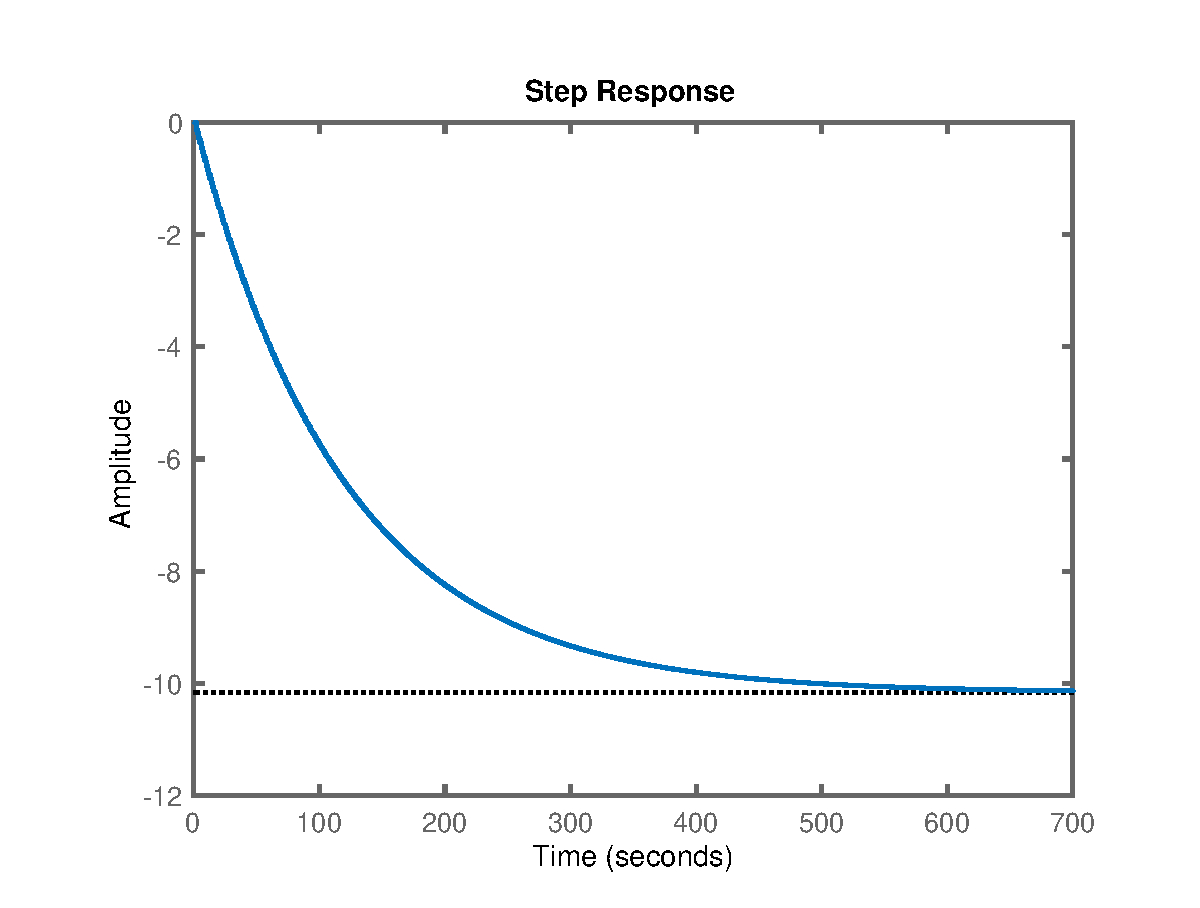
\includegraphics[width=0.5\textwidth]{tf-step-response.eps}
  \caption{Step response for the Eq.~\eqref{tf-synth-controller} describing a stable system for the DC motor plant.}
  \label{tf-step-response}
\end{figure}

Regarding the state-space representation, we have reproduced the stability property for 
the closed-loop control system of a pendulum represented by Eq.~\eqref{ss-synth-controller}. 
%
\begin{equation}
\label{ss-synth-controller}
\begin{split}
x(n+1) &= A x(n) + B u(n)
\\
y(n) &= C x(n) + D u(n), 
\end{split}\
\end{equation}

Where,
%
$$A = \left[\begin{array}{cc}-1.999909737361046&-1.000000000000000\\1&0\end{array}\right],$$
$$B = \left [\begin{array}{c}4\\0\end{array}\right],$$
$$C = \left [\begin{array}{cc}-1.756887232846049&-1.7494556607764090\end{array}\right],$$
$$\quad D = \left [\begin{array}{c}9.8\end{array}\right].$$

For this particular closed-loop control system, the feedback matrix (see Eq.~\eqref{ss-synth-feedback}) generated 
by the \tool also leads to a stable system, as shown in Fig.~\ref{ss-step-response}.
%
\begin{equation}
\label{ss-synth-feedback}
\begin{split}
K &= \left [\begin{array}{cc}-0.5898&-0.1914\end{array}\right]
\end{split}\
\end{equation}

\begin{figure}[ht]
  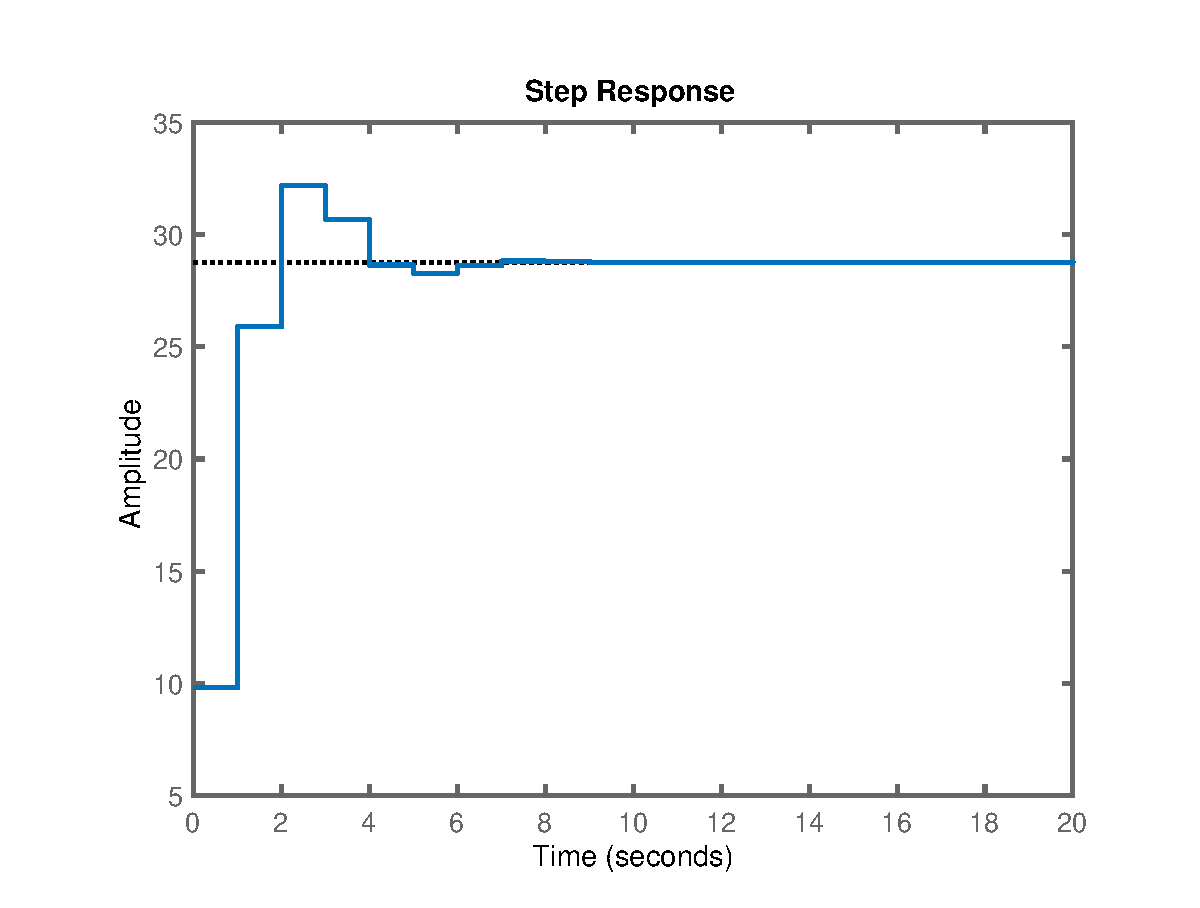
\includegraphics[width=0.5\textwidth]{ss-step-response.eps}
  \caption{Step response for the Eq.~\eqref{ss-synth-controller} describing a stable system for the pendulum plant.}
  \label{ss-step-response}
\end{figure}
 
The digital controllers synthesized by \tool are all stable using the MATLAB step response
as a validation procedure, which means that our results are reliable for control engineers. 
A link to the full experimental environment, including the scripts to reproduce the results, 
all benchmarks, videos, documentation and the tool, is provided online.\footnote{\url{www.dsverifier.org}}

%--------------------------------------
\section{Conclusions}
%--------------------------------------

The \tool can automatically synthesize stable digital controllers for intricate dynamic physical plants, 
represented in MATLAB as a transfer function or a state-space equation using the CEGIS approach. 
In particular, the \tool represents the first fully automated synthesis
tool that is algorithmically and numerically sound, considering various error
sources in the implementation of the digital control algorithm and in the computational 
modeling of plant dynamics~\cite{abate2017,abatecav2017}.
%
Additionally, given the current literature in controller synthesis, there is no other MATLAB toolbox 
for synthesizing stable digital controllers for physical plants, while taking into account all aspects of its 
digital implementation. 
%
As future work, the \tool will perform synthesis of other specifications (e.g., performance) 
and be combined with DSVerifier/DSValidator Toolboxes~\cite{issta2017,dsvalidator} to verify/validate 
other controller properties (e.g., presence of limit cycles). 

\bibliographystyle{IEEEtran}
\bibliography{references} 

\end{document}
